\chapter{Google App Engine.}\label{cap:GAE}
En este apartado de la memoria voy a explicar lo que es, la configuración y como usar la plataforma Google App Engine.

\section{Introducción.}
Google App Engine es una conjunto de apis que proporciona Google para construir tus propias aplicaciones web, que pueden ser alojadas y usadas en su servicio Google App y vendidas en Google Apps Marketplace. Además de alojamiento gratuito Google, ofrecen un dominio, que es: \url{http://nombre\_de\_la\_aplicacion.appspot.com} y una base de datos propietaria de Google que se accede transparentemente a través de la api, gestión de usuarios mediante autentificación con cuentas Google del tipo: \textit{usuario@gmail.com}, autentificación por federación o \textit{openID}.

Además de todas esas características Google proporciona apis para Java, Python y Go, este último un lenguaje experimental del propio Google. Para usar dicha API, Google también da un plugin para Eclipse, en caso de que el lenguaje elegido sea Java, que ayuda al despliegue de la aplicación web, autocompletado y gestión de de las aplicaciones creadas. 
%TODO:En el anexo 1 se puede ver como instalar el puglins para eclipse de google app engine.

En el proyecto solo he usado la API de Google App Engine de Java, por lo que todo lo que puedo comentar es de dicha API, la parte de Python y Go no se han estudiado.

En general el uso de Google App Engine para crear aplicaciones web es idéntico a crear una aplicación web con Java 2 Enterprise Edition (Java2EE), se pueden crear servlet que recogen valores \textbf{GET} o \textbf{POST} y además clases java para hacer operaciones con dichos valores. A su vez para mostrar la infomación se pueden generar archivos \textit{*.jsp}, que son archivos html con bloques o líneas de código java que se introducen con estas etiquetas: $<$\%= línea de código Java \%$>$ o $<$\% Bloque de código Java \%$>$. A parte de archivos \textit{*.java} y \textit{*.jsp}, debemos tener una carpeta llamada \textit{war} en la que tiene que ir toda la información de la aplicación web que queremos deplegar. En dicha carpeta hay varias subcarpetas como pueden ser \textit{css} en la que tiene que ir el estilo de la web o \textit{WEB-INF} en la que están todos los archivos de configuración, como pueden ser los permisos que tenemos que tener para poder acceder al uso de un servlet, si la web tiene conexión https, la configuración de la base de datos, etc.

Para este proyecto se han tenido que desarrollar dos aplicaciones web, una que es un servidor de timestamp y otra que es una aplicación para gestión de las firmas digitales que realice cada usuario. A continuación vamos a explicar en profundida la tecnología usada y ambas aplicaciones web.

\section{Explicación de una aplicación web genérica en Google App Engine.}
En esta parte voy a explicar en profundidad que es un servlet, los archivos de configuración, los archivos \textit{*.jsp} y el resto de archivos necesarios para poder desplegar una aplicación en Google Apps.
 
\subsection{¿Qué es un servlet?.}
Un servlet es la evolución de los antiguos applet, su uso más comun es generar páginas web dinámente con los parámetros que recibe mediante una petición realizada por el navegador web y datos que están almacenados en el servidor web.

Un servlet es un objeto java que tiene que ser ejecutado en un servidor web o contenedor J2EE, que recibe unos parámetros, realiza una o varias acciones y devuelve un resultado que puede ser desde un código html, un JSP que genera dinámicamente un código html, un JSON o una simple cadena de texto.

Los servlets, junto con JSP, son la solución de Oracle a la generación de contenido dinámico equivalente al lenguaje PHP, ASP de Microsoft, Ruby, etc.

Los servlet forman parte de Java Enterprise Edition (JEE) que a su vez es una amplicación de Java Standard Edition (JSE), para usarlos necesita un servidor web que pueda interpretar código java, el más famoso es Apache Tomcat que está desarrollado y mantenido por Apache Foundation, que son los encagardos también de mantener y desarrollar el famoso servidor web Apache, aunque existen otro como JBoss, Jetty o GlassFish, pero como veremos en este proyecto no son los únicos, ya que el propio Google Apps también funciona internamente a base de servlets y JSP.

Para crear un servlet hay que generar una clase java que implemente la interfaz \textit{javax.servlet.Servlet} o que extienda cualquier clase que herede de una clase o que implemente la interfaz anterior, como puede ser \textit{javax.servlet.http.HttpServlet} que es específico para conexiones HTTP. 
Una vez generada la clase hay que implementar el método \textbf{doGet} para peticiones tipo \textbf{GET} o el método \textbf{doPost} para peticiones de tipo \textbf{POST}. En el siguiente trozo se código se puede ver la implementación mas básica de los métodos \textbf{doGet} y \textbf{doPost}, con las llamadas sus respectivas llamadas a \textit{super}.

\begin{lstlisting}[style=Java] 
@Override
protected void doGet(HttpServletRequest req, 
	HttpServletResponse resp) throws ServletException, IOException {
	// TODO Auto-generated method stub
	super.doGet(req, resp);
}

@Override
protected void doPost(HttpServletRequest req, 
HttpServletResponse resp) throws ServletException, IOException {
	// TODO Auto-generated method stub
	super.doPost(req, resp);
}
\end{lstlisting}


Una vez implementados los métodos que se necesiten se pueden usar el parámetro \textit{HttpServletRequest req} para recibir los valores que queramos enviar a la aplicación web y podemos usar \textit{HttpServletResponse resp} para enviar lo que queramos desde una redirección a JSP o una página web a una JSON o cadena de texto. 
Un ejemplo de como se reciben los parámetros sería: 

\begin{lstlisting}[style=Java]  
String num_sec = req.getParameter("sec");
\end{lstlisting}

Y si queremos enviar algo por \textit{HttpServletResponse resp} podríamos usar:

\begin{lstlisting}[style=Java]   
PrintWriter out = resp.getWriter();
out.print(jsonArray);
out.flush();
\end{lstlisting}

Como podemos ver el objeto \textit{resp} nos da la posibilidad de conseguir un objeto \textit{java.io.PrintWriter} por el que podemos enviar lo que necesitemos.

%TODO: añadir la referencia... xD donde pone capítulo proximos xD
La forma de acceder a un servlet mandandole peticiones \textbf{GET} sería la siquiente: \url{https://servertimestamp.appspot.com/search?id=63&texto=Prueba}, como se puede ver la dirección base seria: \url{https://servertimestamp.appspot.com/}, el servlets estaría mapeado internamente en el servidor web, como ya veremos en próximas sección, en la dirección \url{/search} y el primer parámetro va precedido de \url{?id\_parametro} y el resto de \url{\&id\_parametro}. En nuestro ejemplo tendría dos parámetros que son \textit{id} y \textit{texto}, con sus respectivos valores después del =.

El método \textbf{POST} es el utilizado para pasar parámetros por medio de formularios.

\subsection{¿Qué es JSP?.}
JSP es el acrónimo de JavaServer Pages y es una tecnología que ayuda a crear dinámicamente páginas web badas en HTML o XML y es la solución equivalente a PHP de Oracle. En la figura~\ref{fig:modoJSP} se puede observar el proceso que sigue desde que se hace la petición en el navegador hasta que se muestra.

\begin{figure}
  \centering
    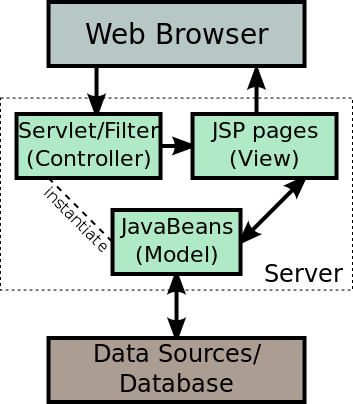
\includegraphics[scale=0.5]{./GoogleAppEngine/imagenes/JSP_Model.png}
  \caption{Modo de interpretación de un archivo JSP}
  \label{fig:modoJSP}
\end{figure}

Un fichero \textit{*.jsp} es la unión de código HTML con código java, el cual es interpretado en el momento de visualización de la página web. Un ejemplo es el siguiente:
 
\begin{lstlisting}[style=HTML]   
<!DOCTYPE html>
<html>
<body>
<table>
<tr>
	<th>ID</th>
	<th>Num sec</th>
	<th>Token de tiempo</th>
	<th>Mensaje</th>
	<th>URL para ver la firma</th>
	<th>Fecha</th>
	<th>Usuario</th>
	<th id="filadestino">Destino</th>
	<th>Verificado?</th>
</tr>

<% for (RowRepositorioGeneral row : rows) {%>
<tr>
	<td><%=row.getId()%></td>
	<td><%= row.getNum_sec()%></td>
	<td><%=row.getToken_tiempo()%></td>
	<td><%=row.getTexto_claro()%></td>
	<td><a href=<%=row.getUrl_firma()%>>URL para ver el token
			de tiempo</a></td>
	<td><%=row.getFecha()%></td>
	<td><%=row.getUsuario()%></td>
	<td id="filadestino"><%=row.getDestino()%></td>
	<td>
		<%
		Boolean confirmado = row.getConfirmado();
		if (!(confirmado == null) && confirmado) {
		%>
		<center>
			<img src="ok.png" />
		</center> <%} else  %>
	</td>
</tr>
<%}%>
</table>
</body>
</html>
\end{lstlisting}

Como se puede ver en este trozo de código este jsp genera una tabla que se rellena dinámicamente con los valores que devuelve un objeto java, se puede observar que se entrelazan trozos de código Java con etiquetas HTML. Si mostramos esta web y acto seguido introducimos otro objeto RowRepositorioGeneral en la estructura, cuando recarguemos la tabla tendrá una fila nueva.

\subsection{La carpeta WAR.}
La carpeta WAR es la carpeta principal para el despliegue de una aplicación web, ya que en ella es donde tienen que ir todos los archivos que necesitemos, desde archivos HTML, CSS, JSP, imágenes, etc. En la figura~\ref{fig:carpetawar} se puede ver un ejemplo de la carpeta WAR de mi aplicación web.

\begin{figure}
  \centering
    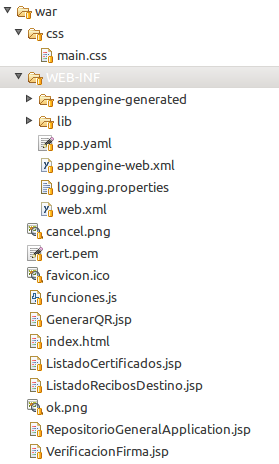
\includegraphics{./GoogleAppEngine/imagenes/carpetawar.png}
  \caption{Carpeta WAR}
  \label{fig:carpetawar}
\end{figure}

Se puede ver las diferentes carpetas y ficheros que la forman. Se ve la carpeta css que contiene los archivos de estilo que la página web usará, también se pueden ver los archivos \textit{web.xml} y \textit{app.yalm} que son archivos de configuración del servidor que se verán en el proximo apartado~\ref{ref_archivos_configuracion_google_app_engine} y además los archivos \textit{jsp} que se usan en la aplicación junto con los archivos \textit{html} y \textit{javascript} que se necesiten.

\subsection{Archivos de configuración.\label{ref_archivos_configuracion_google_app_engine}}
Los principales archivos de configuración son \textit{web.xml} y \textit{app.yalm}, este segundo es solo una forma de escribir de forma más legible el xml, para que nos sea más sencillo escribirlo y leerlo a los humanos.

Un ejemplo de un archivo \textit{web.xml} es el siguiente:

\begin{lstlisting}[language=XML]
<?xml version="1.0" encoding="utf-8"?>
<web-app xmlns:xsi="http://www.w3.org/2001/XMLSchema-instance"
xmlns="http://java.sun.com/xml/ns/javaee"
xmlns:web="http://java.sun.com/xml/ns/javaee/web-app_2_5.xsd"
xsi:schemaLocation="http://java.sun.com/xml/ns/javaee
http://java.sun.com/xml/ns/javaee/web-app_2_5.xsd" version="2.5">

	<servlet>
		<servlet-name>AddRow</servlet-name>
		<servlet-class>pfc.ServletCreateRow</servlet-class>
	</servlet>
	<servlet-mapping>
		<servlet-name>AddRow</servlet-name>
		<url-pattern>/add</url-pattern>
	</servlet-mapping>

	<welcome-file-list>
		<welcome-file>ServerTimestampApplication.jsp</welcome-file>
	</welcome-file-list>
</web-app>
\end{lstlisting}
%TODO: poner la referencia al código si se puede
Como se puede observar en el código se ha definido un servlet que se llamará \textbf{AddRow} que usará la clase \textbf{ServletCreateRow} y que estará mapeado en la dirección web \textbf{/add}, también podemos observar que el fichero que nos mostrará el servidor será \textbf{ServerTimestampApplication.jsp} si entramos a la url principal.

A continuación veremos como es un archivo \textit{app.yalm}:
\begin{lstlisting}[language=YAML]
application: repositoriorecibos
version: 1
runtime: java

handlers:
  - url: /add
    servlet: pfc.ServletCreateRow
    secure: always
welcome_files:
  - RepositorioGeneralApplication.jsp
\end{lstlisting}

Como podemos observar es mucho más fácil de entender y de escribir, el único problema que tienen los archivos YALM es que son sensibles a los espacios en blanco y tabuladores, por lo que hay que tener cuidado al redactarlos. En este archivo se crea un servlet en la ruta \textbf{/add}, que es la clase java \textbf{ServletCreateRow} del paquete \textbf{pfc} y que siempre hay que estar registrado en la aplicación para poder acceder a él. También podemos observar el fichero de bienvenida para cuando accedemos a la aplicación web. 
Al tener el archivo \textit{app.yalm} en la carpeta WEB-INF el parseador de YALM interpreta dicho archivo y genera un archivo \textit{web.xml} que es el que usará el servidor web para su configuración automáticamente.

Para ver todas las opciones de configuración que se pueden modificar en \textit{app.yalm} o en \textit{web.xml} se puede consultar estos enlaces \url{https://developers.google.com/appengine/docs/java/config/}, \url{https://developers.google.com/appengine/docs/java/configyaml/}. En el primero podemos ver todas las opciones configurables de \textit{web.xml} y el la segunda las de \textit{app.yalm}.

\section{Servidor de timestamp.}
En este apartado voy a explicar en profundidad todo lo relacionado con la aplicación de timestamp que he tenido que desarrollar, desde el diseño que se ha seguido hasta los problemas que me han surgido.

En principio me gustaría explicar para que se usa un servidor de timestamp en general. Un servidor de timestamp es un registro donde toda persona puede subir un documento y el servidor guarda ese documento añadiendole la fecha en la que se realizó la subida, dicha aplicación luego ofrece el servicio de consultar a que hora fue subido dicho documento. Un ejemplo podría ser \url{https://seguro.ips.es/servidortimestamp/index.asp} que se puede ver una captura de pantalla en la figura~\ref{fig:server_ips_timestamp}. En dicha captura podemos ver que tiene las opciones básicas de un servidor de timestamping como puede ser generar un sello, consultar su validez, etc. 

\begin{figure}[hbt]
  \centering
    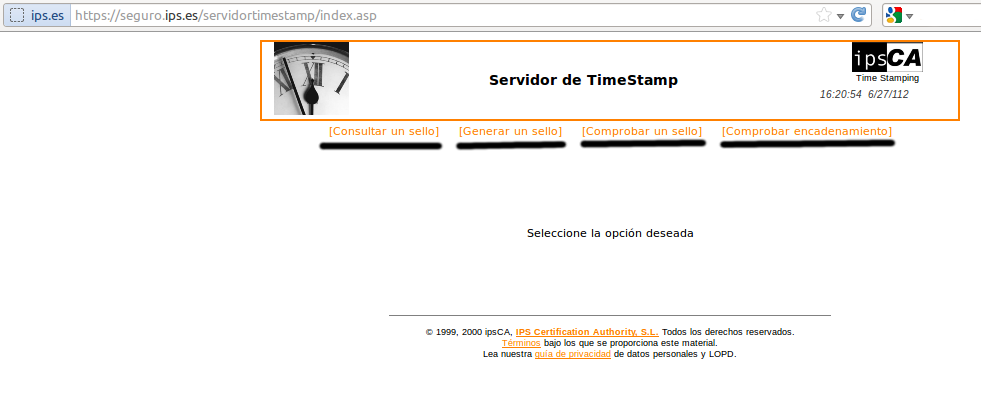
\includegraphics[scale=0.5]{./GoogleAppEngine/imagenes/server_ips_timestamp.png}
  \caption{Servidor Timestamp https://seguro.ips.es}
  \label{fig:server_ips_timestamp}
\end{figure}

La veracidad de que el sellado de dicho documento fue en el instante que dice ser, depende de la confianza que se tenga en ese servicio. Es similar a cuando se necesita que te sellen un documento físico, que dependiendo de para quien lo necesite, necesitas que lo firme un notario o un empleado público si es para una entidad pública. Normalmente suelen existir servidores de timestamping en los que se tiene confianza y los documentos sellados se consideran verdaderos.

Existen tres modelos principales de servidor de timestamping que son los siguientes:
\begin{itemize}
\item \textbf{Solución Arbitrada básica:} En esta solución el usuario que quiere sellar algo mandaría una copia del documento que quiere sellar a la entidad de sellado, que a su vez pondría el sello de tiempo y a su vez guardaría una copia de dicho documento, este es el modelo mas parecido a la vida real. Esta solución tiene un par de problemas grandes como puede ser que la privacidad del documento se pierde, tenemos que tener en cuenta que el servidor de timestamping puede estar en España, EEUU o en cualquier otro país y a su vez la base de datos para almacenar todos los documentos tiene que ser enorme, por lo que almacenar todos los documentos nos puede acarrear muchos problemas.

\item \textbf{Solución Arbitrada avanzada:} Esta solución es una evolución de la anterior, en ella el cambio que se hace es que el usuario que quiere que le sellen el documento manda el hash de dicho documento, un hash es el resultado de una función unidireccional que recibe un documento y devuelve un valor único, teniendo dicho valor no se puede saber el documento original, pero dicho documento siempre creará ese valor único, y la entidad solo tendría que almacenar dicho hash junto con el sello de tiempo que se ha generado. Esta solución no tiene los inconvenientes de la anterior, ya que el tamaño de los documentos se reduciría a unos pocos bytes, y la privacidad del documento no se ve comprometida. El problema que si persiste es que el usuario conozca a la entidad de certificación y puedan generar timestamp falsos, pero este problema ya va dentro de la confianza que queramos darle a ese servicio. Suponemos que si es un servicio oficial y serio este problema no va a suceder, de todas formas existen otras soluciones que arreglan este problema.

\item \textbf{Solución Arbitrada avanzada y distribuida:} Esta forma consigue arreglar el problema de la anterior que se produzca un uso fraudulento del timestamping es usando varias entidades de timestamping, por lo que el usuario mandaría el hash a varias entidades de sellado y el usuario guarde los reguardos que están firmados digitalmente de todas las entidades. Así si en una hay un problema tiene varias copias que certifican que se selló dicho instante.

\item \textbf{Solución mediante enlaces:} Esta solución es la mas compleja y a su vez la que soluciona todos los problemas anteriores, además tiene la ventaja de que no tiene que usar multitud de entidades de certificación. Consiste en que cuando un usuario quiere sellar algo, manda el hash del documento, la entidad añade el número de serie del documento anterior, el timestamp y lo firma digitalmente, entonces el problema de que se introduzcan valores fraudulentos por mitad se anula, ya que cada recibo está enlazado con el anterior.
\end{itemize}

En nuestro caso hemos desarrollado un servidor de timestamping en su versión solución arbitrada avanzada.

A continuación voy a explicar la aplicación web, los servlets que la componen y sus funciones.

\subsection{Explicación de la aplicación web.}
%TODO: falta explicar como funciona la BD...
En este capítulo voy a explicar todas las partes que componen la aplicación web que he desarrollado para la implementación del servidor timestamp.

En la figura~\ref{fig:paquete_pfc} se puede ver las clases que forman el paquete \textit{pfc}.

\begin{figure}
  \centering
    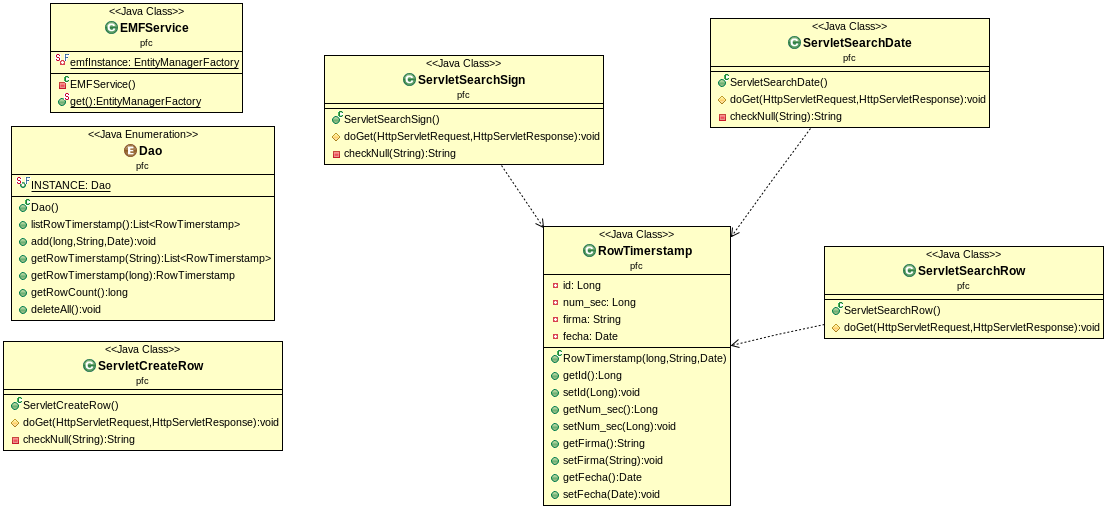
\includegraphics[scale=0.5]{./GoogleAppEngine/imagenes/UML_pfc.png}
  \caption{Detalles del paquete pfc}
  \label{fig:paquete_pfc}
\end{figure}

A continuación voy a explicar una a una las clases desarrolladas.

\begin{description}
\item \textbf{Dao.java: \label{prueba}} Esta clase es la encargada de todos los accesos a la base de datos, desde insercción, borrado y listado de las filas, hasta consultas que se necesiten hacer. Se puede observar que las consultas que son de listado de columnas se ejecutan con una sentencia SQL, un ejemplo es la siguiente:
\begin{lstlisting}[style=Java]
EntityManager em = EMFService.get().createEntityManager();
Query q = em.createQuery("select t from RowTimerstamp t where t.num_sec = :num_sec");
q.setParameter("num_sec", id);
RowTimerstamp RowTimerstamps = (RowTimerstamp)q.getSingleResult();
\end{lstlisting}

Pero las consultas que implican borrado o inclusión de filas no se realizan con sentencias SQL convencionales, se añaden con métodos que proporciona la API, un ejemplo es el siguiente:
\begin{lstlisting}[style=Java]
EntityManager em = EMFService.get().createEntityManager();
RowTimerstamp RowTimerstamp = new RowTimerstamp(num_sec, firma, fecha);
em.persist(RowTimerstamp);
em.close();
\end{lstlisting}

\item \textbf{RowTimerstamp.java:} En esta clase se diseña el formato de las filas de la base de datos, que como se ha explicado anteriormente no se crea con sentencias SQL, se usa un modelo de programación llamado JPA. Para dicho modelo hay que crear una clase que contenga como variables de clase las columnas de la tabla de la base de datos. Como podemos ver mediante anotaciones Java se le indica que campo es la clave primaría, también se puede indicar que ese campo es autoincrementado y otras opciones que habría que indicar en la creación de la tabla.   

\begin{lstlisting}[style=Java]
@Id
@GeneratedValue(strategy = GenerationType.SEQUENCE)
private Long id;
private Long num_sec;
private String firma;
private Date fecha;
\end{lstlisting}

Se puede ver que el campo id será la clave primaría que se indica con \textit{@id} y que es autoincremental, a su vez también podemos ver el resto de datos que se van a guardar, el campo \textit{num\_sec} es el número de secuencia, ya que el campo \textit{@id} lo usa la base de datos para organizarse ella, el campo \textit{firma} es hash firmado por el usuario y que se quiere tener constancia de que se subío en la fecha que indica el campo \textit{fecha}.
El resto de métodos que tiene esta clase es un contructor, getter para consultar los campos y setter para insertar valores.

\item \textbf{ServletCreateRow.java:} Esta clase es un servet que se encagar de recibir todos los parámetros necesarios y añadirlos a la base de datos. Al recibir los parámetros mediante \textbf{GET} tiene que implementar el método \textit{doGet}, casi todos los servlets implementados en el proyecto mandan los parámetros mediante \textbf{GET}. La forma de recibir parámetros es la siguiente:

\begin{lstlisting}[style=Java]
String firma = req.getParameter("firma");
\end{lstlisting}

El resto de parámetros que se necesitan se generan en el servidor para que no puedan ser falseados, como es el número de secuencia y la fecha.

Si la insercción se produce correctamente se devuelve una cadena que tiene el siguiente formato: ``ok;;num\_sec;;fecha" que será interpretado en la aplicación android y que parseará dicha cadena para conseguir los valores que necesitemos.

\item \textbf{ServletDeleteAll.java:} Es un servlet ``secreto" que se usa para borrar todas las filas del servidor, cosa que no se debería poder para no poder falsear los datos introducidos en el servidor de timestamp. Hay que llamarlo con un parámetro que es \textbf{borrar} con valor \textbf{5}.

\item \textbf{ServletSearchDate.java:} Es un servlet que devuelve una cadena con la fecha de una fila que tiene el número de secuencia que se le pasa en el parámetro \textbf{token}.

\item \textbf{ServletSearchRow.java:} Es un servlet que devuelve una página web donde se puede observar en una única columna toda la infomación almacenada que corresponde con el número de secuencia que se le pasa en el parámetro \textbf{id}. La forma de hacerlo es la siguiente:

\begin{lstlisting}[style=Java]
PrintWriter pw = resp.getWriter();
pw.print("<!DOCTYPE html>");
pw.print("<html><head><title>Lista Time Stamp</title><link rel=\"stylesheet\" type=\"text/css\" " +
		"href=\"css/main.css\"/> <meta charset=\"utf-8\"> </head>");
pw.print("<body><table><tr><th>ID</th><th>Num sec</th><th>Firma</th><th>Date</th></tr><tr> " +
		"<td>"+ row.getId() +"</td><td>"+ row.getNum_sec() +"</td><td>"+ row.getFirma() +"</td><td>" +
		row.getFecha() + "</td></tr> </table></body>");
pw.flush();
\end{lstlisting}

Como se puede ver se crea una tabla en una web que su fila se generan dinámicamente dependiendo del número de secuencia que se le pase.

\item \textbf{ServletSearchSign.java:} Es un servlet que devuelve una cadena con la firma que corresponde al número de secuencia que se pasa por el parámetro \textbf{token}.
\end{description}
%TODO: falta los jsp

\section{Servidor de registro de firmas.}
El servidor de registro de firmas que hemos desarrollado es una aplicación web en la que se pueden consultar las firmas que tu has realizado, las firmas en las que el destinatario eres tú, gestión del certificado de clave pública, verificar una firma, exportar una cadena con la que cualquier persona puede mirar si la firma que has realizado es válida para comprobaciones en caso de algún problema, y generar códigos QR para que que alguien que lo necesite pueda firmarlo.

El sistema de gestión de usuarios la proporciona google, y para entrar en la aplicación web hay que tener una cuenta de google, si no se produce una redirección a la página de logueo que se puede ver en la figura~\ref{fig:logueoRepoGeneral}.
\begin{figure}
  \centering
    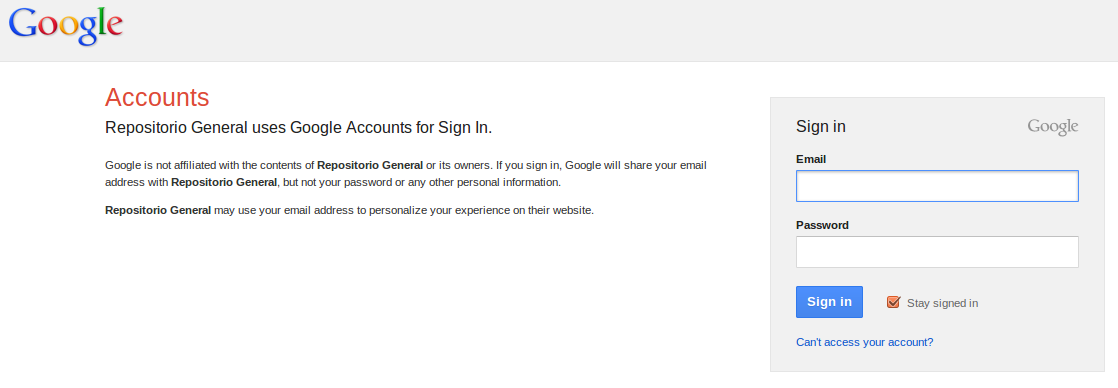
\includegraphics[scale=0.5]{./GoogleAppEngine/imagenes/login_repositorio_general.png}
  \caption{Login en Repositorio General}
  \label{fig:logueoRepoGeneral}
\end{figure}
La parte de la seguridad de los usuarios, logueo y mantenimiento de las base de datos ya las proporciona el mismo Google.

La aplicación web se puede ver en la figura~\ref{fig:repositorio_general}.
\begin{figure}[gae]
  \centering
    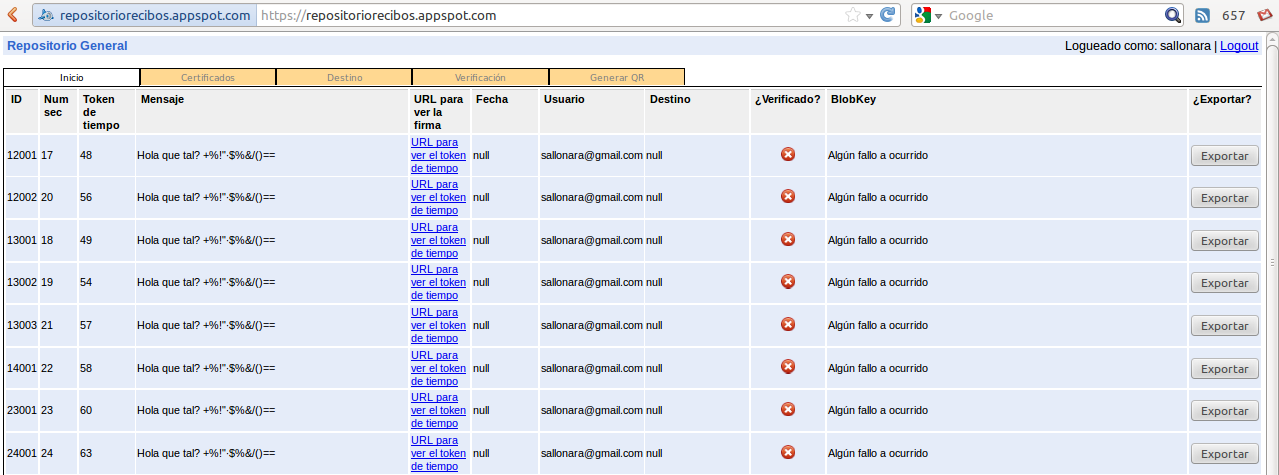
\includegraphics[scale=0.5]{./GoogleAppEngine/imagenes/repositorio_general.png}
  \caption{Repositorio General}
  \label{fig:repositorio_general}
\end{figure}

La aplicación tiene varias pestañas, que se explicarán posteriormente cuando expliquemos cada archivo \textit{*.jsp}, pero principalmente cada una de ellas se encarga de hacer una de las funciones que hemos comentado anteriormente.

\subsection{Explicación de la aplicación web.}
%TODO: falta explicar como funciona la BD...
En la figura~\ref{fig:clasesReposotorioGeneral} se puede ver las clases que forman el paquete \textit{pfc} de la aplicación web repositorio general.

\begin{figure}
  \centering
    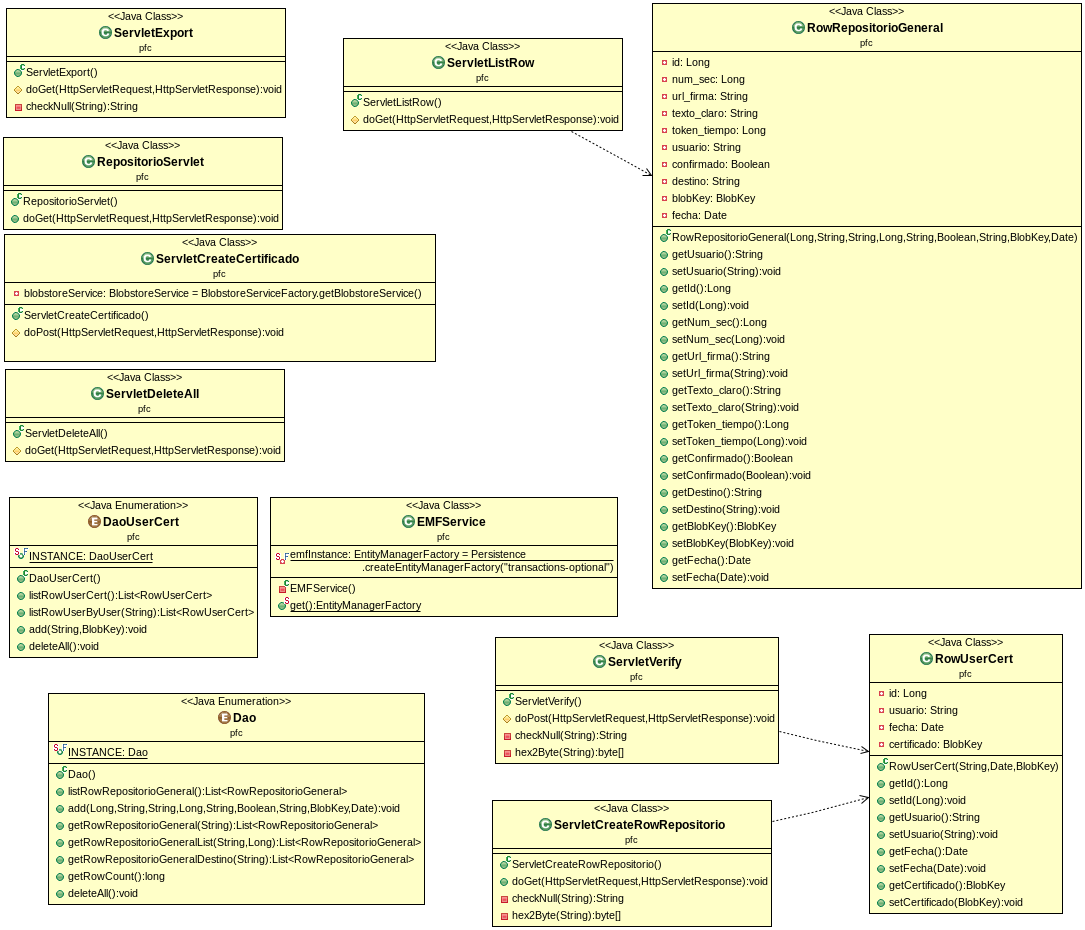
\includegraphics[scale=0.5]{./GoogleAppEngine/imagenes/UML_repositorio.png}
  \caption{Detalles de las clases Repositorio General.}
  \label{fig:clasesReposotorioGeneral}
\end{figure}

A continuación vamos a explicar una a una las clases desarrolladas.

\begin{description}
\item \textbf{Dao.java:} Al igual en el servidor de timestamp esta clase es la encargada de hacer todas operaciones contra la base de datos. Para mas información mirar el apartado~\ref{prueba}.

\item \textbf{DaoUserCert.java:} En este aplicación hemos utilizado dos bases de datos, una para guardar las firmas y otra para guardar los certificados de clave pública que se necesitan para verificar si una firma es correcta o no. Esta clase es la encargada de todos los accesos, tanto inserciones como consultas, a dicha tabla. 

\item \textbf{RowRepositorioGeneral.java:} Esta es la clase con la que se crea la tabla en la que se almacenan las firmas de los usuario, tiene los siguientes campos:  

\begin{lstlisting}[style=Java]
@Id
@GeneratedValue(strategy = GenerationType.SEQUENCE) //	 GenerationType.IDENTITY
private Long id;
private Long num_sec;
private String url_firma;
private String texto_claro;
private Long token_tiempo;
private String usuario;
private Boolean confirmado;
private String destino;
private BlobKey blobKey;
private Date fecha;
\end{lstlisting}

Tiene una clave primaría que es \textit{id} que es usada por Google internamente para el almacenado de la información, \textit{num\_sec} es el número de secuencia dentro la tabla que va incrementandose automáticamente, \textit{url\_firma} es la dirección en la cual se puede consultar la firma del texto en claro que está en el campo \textit{texto\_claro}. También se guarda el \textit{token\_tiempo} que es el \textit{num\_sec} de en la aplicación web del servidor de timestamp. La columna \textit{usuario} almacena el usuario que ha subido la firma, y en La columna \textit{destino} se guarda a quien va dirigido la firma, ya que todas firmas tienen un destinatario. En la columna \textit{blobkey} se guarda la referencia al certificado de clave pública que estaba en activo cuando fue subido a la aplicación web, la columna \textit{confirmado} puede valer true or false e indica si al subir la firma se pudo verificar y el texto en claro coincidía con el texto cifrado, en \textit{fecha} está la fecha en la que se almacenó.

\item \textbf{RowUserCert.java:} Esta clase es la encagargada de crear la tabla que usamos para guardar los archivos con la clave pública.
%TODO: poner el tipo de archivo que necesitamos usar y esas cosas.
Los campos que usaremos para almacenarlos serán los que se pueden ver en 

\begin{lstlisting}[style=Java]
@Id
@GeneratedValue(strategy = GenerationType.SEQUENCE)
private Long id;
private String usuario;
private Date fecha;
private BlobKey certificado;
\end{lstlisting}

Como podemos observar el campo \textit{id} será la clave pública y como hemos explicado será usado por la base de datos de Google para autogestión de las filas, el campo \textit{usuario} guardará una cadena con el email de la persona que ha subido ese archivo, el campo \textit{fecha} es la fecha en la que se subió el archivo, dicho campo se usará para comprobar que no se puedan falsear firmas, con varias comprobaciones y para anular certificados en caso de perdidas o que se necesite reemplazarlo, \textit{certificado} es un campo del tipo \textbf{BlobKey} que es como la ruta al archivo de certificado.

\end{description}
A continuación vamos a explicar los diferentes servlets que hemos desarrollado para la aplicación web.

\begin{description}
\item \textbf{ServletCreateCertificate.java:} Este servlet es el encargado de añadir a la base de datos el certificado de clave pública. Es usado en la pestaña de certificados de la aplicación web y es llamado cuando se pulsa subir certificado. Se puede observar el botón subir certificado en la figura~\ref{fig:pestanhaCertificados}.

\begin{figure}
  \centering
    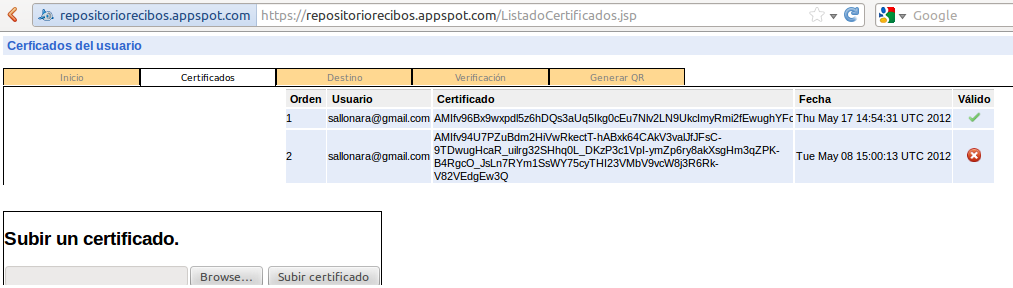
\includegraphics[scale=0.5]{./GoogleAppEngine/imagenes/certificadosRepositorioGeneral.png}
  \caption{Pantallazo de la pestaña certificados.}
  \label{fig:pestanhaCertificados}
\end{figure}

\item \textbf{ServletCreateRowRepositorio.java:} Este servlet está mapeado en la dirección: \url{https://repositoriorecibos.appspot.com/add} y recibe los siguientes parámetros: \textit{texto}, \textit{url\_firma}, \textit{token}, \textit{destino} y \textit{fecha}. Es el encargado de añadir una fila por cada llamada a dicha dirección, a dicho dirección no hay forma de acceder desde la aplicación web, solo se pueden comprobar las firmas ya introducidas. A su vez antes de introducir la fila comprueba que la firma se puede validar y marca como verdadero o falso la columna verificado que posteriormente en el archivo \textit{RepositorioGeneralApplication.jsp} se cambiará por una imagen para hacer la verificación más visual. Si se hemos podido insertar la fila, el servlet devuelve la cadena \textbf{OK}, si no se devuelven varias cadenas con los fallos que se han producido.

\item \textbf{ServletDeleteAll.java:} Servlet ``secreto" que borra todas las filas de firmas almacenadas, hay que llamarlo con un parámetro que es \textit{borrar} con valor \textit{7}

\item \textbf{ServletExport.java:} Este servlet es el encargado de exportar una fila de nuestras filas para que otra persona pueda comprobar si es válida. Este servlet es llamado cuando se pulsa el botón exportar de la pestaña principal de la aplicación web. Se puede observar en la figura~\ref{fig:botonExportar}

\begin{figure}
  \centering
    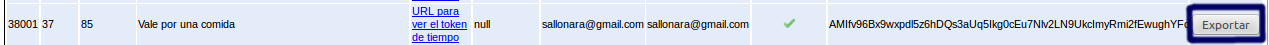
\includegraphics[scale=0.5]{./GoogleAppEngine/imagenes/botonExportar.png}
  \caption{Detalle del botón exportar.}
  \label{fig:botonExportar}
\end{figure}

El servlet recibe los siguiente parámetros:

\begin{lstlisting}[style=Java]
String mensaje = checkNull(req.getParameter("mensaje"));
String url_firma = checkNull(req.getParameter("token"));
String id_blob = checkNull(req.getParameter("id_blob"));
String user = checkNull(req.getParameter("usuario"));
\end{lstlisting}

Una vez se tienen esos parámetros creamos una cadena de texto en la que unimos los siguiente campos y cada parámetro va separado por el separador: \textit{;/:}.
\begin{lstlisting}[style=Java]
String cadACodificar = mensaje + ";/:" + url_firma + ";/:" + id_blob + ";/:" + user;
\end{lstlisting}

Acto seguido codificamos la cadena con \textbf{Base64}, que es una forma simple de codificar los caracteres para que no viajen en texto claro.
\begin{lstlisting}[style=Java]
String cadCodificada = Base64.encode(cadACodificar.getBytes("UTF-8"));
\end{lstlisting}

También añadimos unos limitadores para que cuando tengamos que decodificar ese mensaje podamos saber donde empiezan y donde termina la exportación.
\begin{lstlisting}[style=Java]
pw.println("BEGIN EXPORT");
pw.println("--------------------------");
pw.println(cadCodificada);
pw.println("--------------------------");
pw.println("END EXPORT");
\end{lstlisting}

\item \textbf{ServletListRow.java:} Este servlet es el encargado en devolver todas las filas de la tabla que pertenecen a un usuario. La forma de hacerlo es la siguiente, primero se identifica el usuario con el que se ha logueado de esta forma:

\begin{lstlisting}[style=Java]
UserService userService = UserServiceFactory.getUserService();
User user = userService.getCurrentUser();
\end{lstlisting}

Una vez se consigue el usuario se llama a la función \textit{public List<RowRepositorioGeneral> getRowRepositorioGeneralList(String userId, Long num\_sec)} de la clase \textit{Dao.java}, esta última función nos devuelve una lista con todas las filas. Al llamar al servlet le pasaremos el último número de secuencia que tenemos guardado en el telefono móvil, para así agilizar las transferencias de datos, de esta forma solo nos devolverá las filas nuevas. La forma de devolvernos las filas será en un JSONArray, que es un objeto que dentro contiene varios objetos JSON\footnote{Para saber que es un objeto JSON pueden consultar los siguientes enlaces: \url{http://www.json.org/} o \url{http://en.wikipedia.org/wiki/JSON}}.

La creación de los objetos JSON la realizamos de la siguiente forma:
\begin{lstlisting}[style=Java]
JSONObject jsonObject = new JSONObject();

jsonObject.put("num_sec", rowRepositorioGeneral.getNum_sec().toString());
jsonObject.put("texto", rowRepositorioGeneral.getTexto_claro());
jsonObject.put("url_firma", rowRepositorioGeneral.getUrl_firma());
jsonObject.put("token_tiempo", rowRepositorioGeneral.getToken_tiempo().toString());
jsonObject.put("usuario",rowRepositorioGeneral.getUsuario());
jsonObject.put("fecha", rowRepositorioGeneral.getFecha().toString());
jsonObject.put("verificado", rowRepositorioGeneral.getConfirmado().toString());
jsonObject.put("destino", rowRepositorioGeneral.getDestino());
\end{lstlisting}

Ese objeto JSON se añade un objeto JSONArray que a su vez es el que devolveremos como respuesta al final de la ejecución de nuestro servlet y que espera la aplicación android que lo ha pedido.

\item \textbf{ServletVerify.java:} Este servlet es el utilizado en la pestaña verificar de nuestra aplicación web, como se puede observar en la figura~\ref{fig:pestanhaVerificar}

\begin{figure}
  \centering
    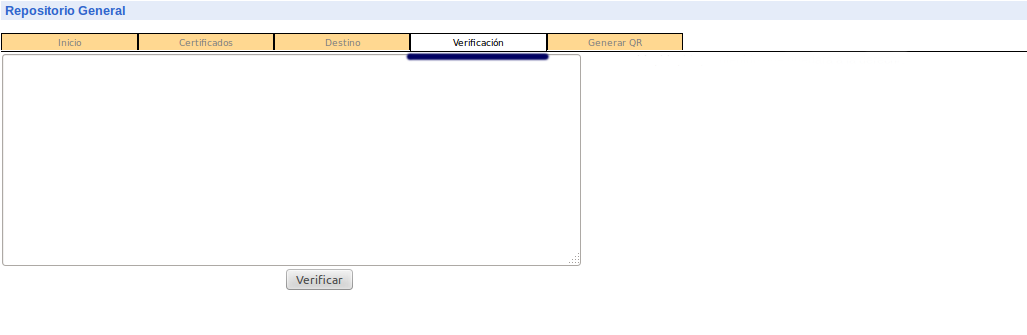
\includegraphics[scale=0.5]{./GoogleAppEngine/imagenes/pestanhaVerificar.png}
  \caption{Detalle de la pestaña verificación.}
  \label{fig:pestanhaVerificar}
\end{figure}

Como podemos observar hay un cuadro de texto para introducir la cadena que devolvería al pulsar el botón exportar. Cualquier usuario puede verificar si una firma es correcta o no. En este servlet se hace el proceso contrario que hicimos en exportar, quitamos los indicadores de inicio y final de exportación, desencriptamos la cadena en Base64 y hacemos varias comprobaciones. Comprobamos que en la fecha en la que se firmó el certificado era válido y que no habiamos revocado ese certificado, también se comprueba que no fuera reemplazado por otro certificado antes de su expiración, ya que entonces la firma no sería válida. También comprobamos la integridad del mensaje, que la cadena no esté mal formada y que siga el formato que hemos obligado anteriormente.
\end{description}

Los archivos \textit{*.jsp} que hemos creado en su mayoría solo rellenan tablas dinámicamente haciendo llamadas a funciones de la clase \textit{Dao.java}. Solo habría uno que no realiza esas funciones que es el siguiente:
\begin{description}
\item \textbf{GenerarQR.jsp:} Este archivo JSP es el que se muestra en la pestaña \textit{Generar QR}, se puede ver en la figura~\ref{fig:pestanhaQR}. Su función es generar un código QR para que pueda ser leido por la aplicación del móvil. Hay que rellenar los campos de destino y el texto que queremos que firme dicha persona. Al darle a \textit{Generar código QR} se hace una llamada a la API Google Chart y se genera un código QR que contiene dichas cadenas y se muestra en la parte de la derecha, como se puede ver en la figura~\ref{fig:codigoQR}.

\begin{figure}
  \centering
    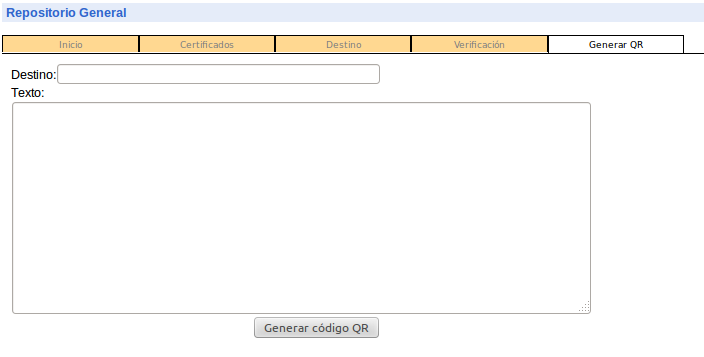
\includegraphics[scale=0.5]{./GoogleAppEngine/imagenes/pestanhaQR.png}
  \caption{Pestaña para generar el código QR.}
  \label{fig:pestanhaQR}
\end{figure}

\begin{figure}
  \centering
    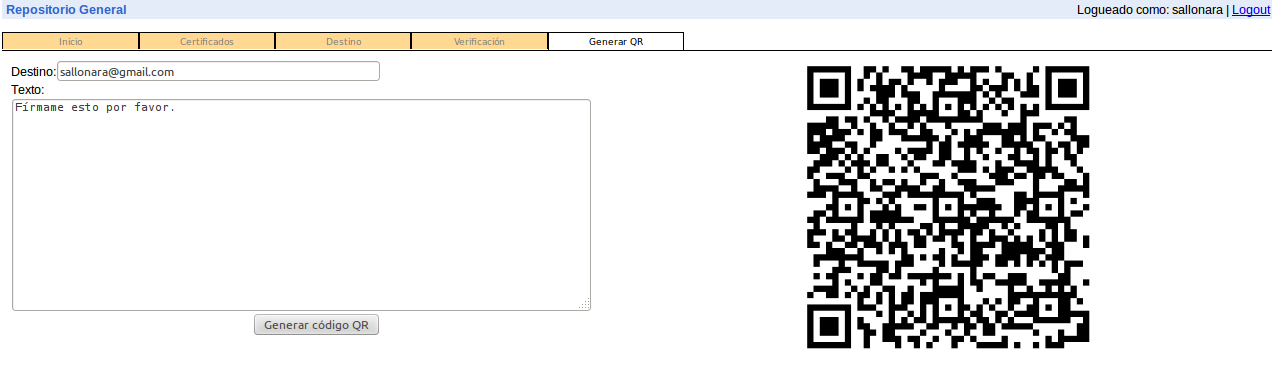
\includegraphics[scale=0.5]{./GoogleAppEngine/imagenes/codigoQR.png}
  \caption{Pestaña con el código QR generado.}
  \label{fig:codigoQR}
\end{figure}

\end{description}


